%!TEX program = xelatex

\documentclass[a4paper, openany, oneside]{memoir}
\usepackage[no-math]{fontspec}
\usepackage{pgfplots}
\pgfplotsset{compat=newest}
\usepackage{commath}
\usepackage{mathtools}
\usepackage{amssymb}
\usepackage{amsthm}
\usepackage{booktabs}
\usepackage{mathtools}
\usepackage{xcolor}
\usepackage[separate-uncertainty=true, per-mode=symbol]{siunitx}
\usepackage[noabbrev, capitalize]{cleveref}
\usepackage{listings}
\usepackage[american inductor, european resistor]{circuitikz}
\usepackage{amsmath}
\usepackage{amsfonts}
\usepackage{ifxetex}
\usepackage[dutch,english]{babel}
\usepackage[backend=bibtexu,texencoding=utf8,bibencoding=utf8,style=ieee,sortlocale=en_GB,language=auto]{biblatex}
\usepackage[strict,autostyle]{csquotes}
\usepackage{parskip}
\usepackage{import}
\usepackage{standalone}
\usepackage{hyperref}
%\usepackage[toc,title,titletoc]{appendix}

\ifxetex{} % Fonts laden in het geval dat je met Xetex compiled
    \usepackage{fontspec}
    \defaultfontfeatures{Ligatures=TeX} % To support LaTeX quoting style
    \setromanfont{Palatino Linotype} % Tover ergens in Font mapje in root.
    \setmonofont{Source Code Pro}
\else % Terug val in standaard pdflatex tool chain. Geen ondersteuning voor OTT fonts
    \usepackage[T1]{fontenc}
    \usepackage[utf8]{inputenc}
\fi
\newcommand{\references}[1]{\begin{flushright}{#1}\end{flushright}}
\renewcommand{\vec}[1]{\boldsymbol{\mathbf{#1}}}
\newcommand{\uvec}[1]{\boldsymbol{\hat{\vec{#1}}}}
\newcommand{\mat}[1]{\boldsymbol{\mathbf{#1}}}
\newcommand{\fasor}[1]{\boldsymbol{\tilde{\vec{#1}}}}
\newcommand{\cmplx}[0]{\mathrm{j}}
\renewcommand{\Re}[0]{\operatorname{Re}}
\newcommand{\Cov}{\operatorname{Cov}}
\newcommand{\Var}{\operatorname{Var}}
\newcommand{\proj}{\operatorname{proj}}
\newcommand{\Perp}{\operatorname{perp}}
\newcommand{\col}{\operatorname{col}}
\newcommand{\rect}{\operatorname{rect}}
\newcommand{\sinc}{\operatorname{sinc}}
\newcommand{\IT}{\operatorname{IT}}
\newcommand{\F}{\mathcal{F}}

\newtheorem{definition}{Definition}
\newtheorem{theorem}{Theorem}


\DeclareSIUnit{\voltampere}{VA} %apparent power
\DeclareSIUnit{\pii}{\ensuremath{\pi}}

\hypersetup{%setup hyperlinks
    colorlinks,
    citecolor=black,
    filecolor=black,
    linkcolor=black,
    urlcolor=black
}

% Example boxes
\usepackage{fancybox}
\usepackage{framed}
\usepackage{adjustbox}
\newenvironment{simpages}%
{\AtBeginEnvironment{itemize}{\parskip=0pt\parsep=0pt\partopsep=0pt}
\def\FrameCommand{\fboxsep=.5\FrameSep\shadowbox}\MakeFramed{\FrameRestore}}%
{\endMakeFramed}

% Impulse train
\DeclareFontFamily{U}{wncy}{}
\DeclareFontShape{U}{wncy}{m}{n}{<->wncyr10}{}
\DeclareSymbolFont{mcy}{U}{wncy}{m}{n}
\DeclareMathSymbol{\Sha}{\mathord}{mcy}{"58}
\addbibresource{../../../includes/bibliography.bib}

\title{Introduction}

\author{W.P. Bruinsma \and R.P. Hes \and H.J.C. Kroep \and T.C. Leliveld \and W.M. Melching \and T.A. aan de Wiel}

\raggedbottom

\begin{document}
\section{System overview}
Our approach consists of several components, which all work together to achieve the functionality specified in the previous section. The components are as follows.

\begin{description}
    \item[Sampling] Sampling consists of applying sampling techniques to the signal whose spectrum has to be sensed. Sampling is not part of the system, but forms an interface between the the signal and the toolkit.
    \item[Reconstruction] Reconstruction analyses the sampled signal. Reconstruction has knowledge of the used sampling technique in sampling to perform this analysis.
    \item[Detection] Detection performs the identification of signals based on the analysis of the reconstruction. Detection and reconstruction closely work together.
\end{description}

The modules are depicted in \cref{fig:overview}. They will be discussed more detailled in the following subsections.
\begin{figure}
    \centering
    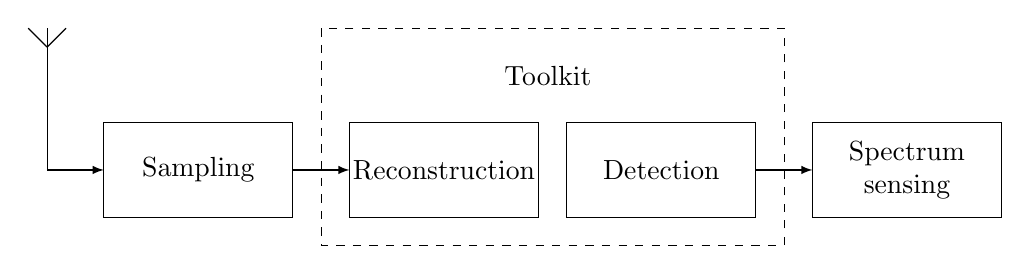
\begin{tikzpicture}[scale=1.2]

    \draw  (-0.6,1.5) rectangle (1.4,0.5) node[pos=.5]{Sampling};
    \draw  (2,1.5) rectangle (4,0.5) node[pos=.5]{Reconstruction};
    \draw  (4.3,1.5) rectangle (6.3,0.5) node[pos=.5]{Detection};
    \draw  (6.9,1.5) rectangle (8.9,0.5) node[pos=.5,text width=2cm, align=center]{\centering Spectrum sensing};
    \draw  [dashed] (1.7,2.5) rectangle (6.6,0.2);
    \node at (4.1,2) {Toolkit};

    \draw [>=latex,->] (1.4,1) -- (2,1);
    \draw [>=latex,->] (6.3,1) -- (6.9,1);
    \draw [>=latex,->] (-1.2,1) -- (-0.6,1);

    \draw (-2+0.8,1) -- (-2+0.8,2.5);
    \draw (-1.8+0.8,2.5) -- (-2+0.8,2.3);
    \draw (-2.2+0.8,2.5) -- (-2+0.8,2.3);
    \end{tikzpicture}
    \caption{System overview. The system components are shown.}
    \label{fig:overview}
\end{figure}


\subsection{Sampling}
The first step in high-performance real-time wideband spectrum sensing is sampling the signal whose spectrum has to be sensed. Conventionally, this is done by making use of uniform sampling at the Nyquist frequency\footnote{The Nyquist frequency is the minimum frequency at which a signal can be sampled without distorting the signal. The Nyquist frequency is twice the highest frequency present in the signal.}. This ensures that the signal can be reconstructed after sampling. However, the Nyquist frequency becomes very high when one wants to sense a very large bandwidth, which is specified in the specifications. Since the Nyquist frequency becomes very high, to sense the specturm, one has to use hardware which supports such high Nyquist frequencies. This hardware can be very expensive.

We investigate alternative sampling techniques which are non-uniform sampling techniques. These techniques can be implemented by making use of multiple sampling devices, also called samplers. Non-uniform sampling is discussed in \cref{cha:sampling} and non-uniform sampling techniques are discussed in \cref{cha:sampling_methods}.

\subsection{Reconstruction}
Noise is omnipresent. Even when a signal is present, this signal is contaminated with noise. The goal of our system is to determine which frequencies contain signal distinct from noise. It can be shown that this decision problem is solved optimally by evaluating the signal power \cite{axell2012spectrum}. Therefore, we look at the signal power per frequency to decide per frequency whether a signal present or not. The signal power per frequency is also called the power spectral density.

Sampling makes use of non-uniform sampling techniques. As a consequence, we may not be able to reconstruct the sampled signal. However, reconstruction of the sampled signal is not necessary, since we only want to determine which frequencies contain signal and which do not. Therefore, reconstruction analyses the sampled signals and only reconstructs the power spectral density of this signal, which we argued to be important for identifying signals. This reconstruction will be done real-time. Reconstruction is discussed in \cref{cha:reconstruction}.

\subsection{Detection}
In the previous paragraph we saw that reconstruction reconstructs the power spectral density of the sampled signal. Detection then analyses this power spectral density, and decides per frequency whether a signal is present or not. This decision process is not based upon which kind of information is encoded in those frequencies, but only determines if \textit{any} kind of information is present. After it is determined at which frequencies signals are present, the spectrum sensing process is complete. Detection is discussed in \cref{cha:detection}.


% The detection process operates on the autocorrelation as provided by the \emph{reconstructor}. By calculating the power spectral density from the autocorrelation we obtain the expected average power per frequency. This information can be used by the detector to itself is not concerned about the information encoded in those signals, but only in which frequency bands they occupy. 


\end{document}